\section{Proposed Architecture}
A better zoomable representation of these diagrams can be found in the github repository of this project in /doc/pflichtenheft/pics, where also the xml sources are.
\subsection{Overview}

\hspace{-3cm} 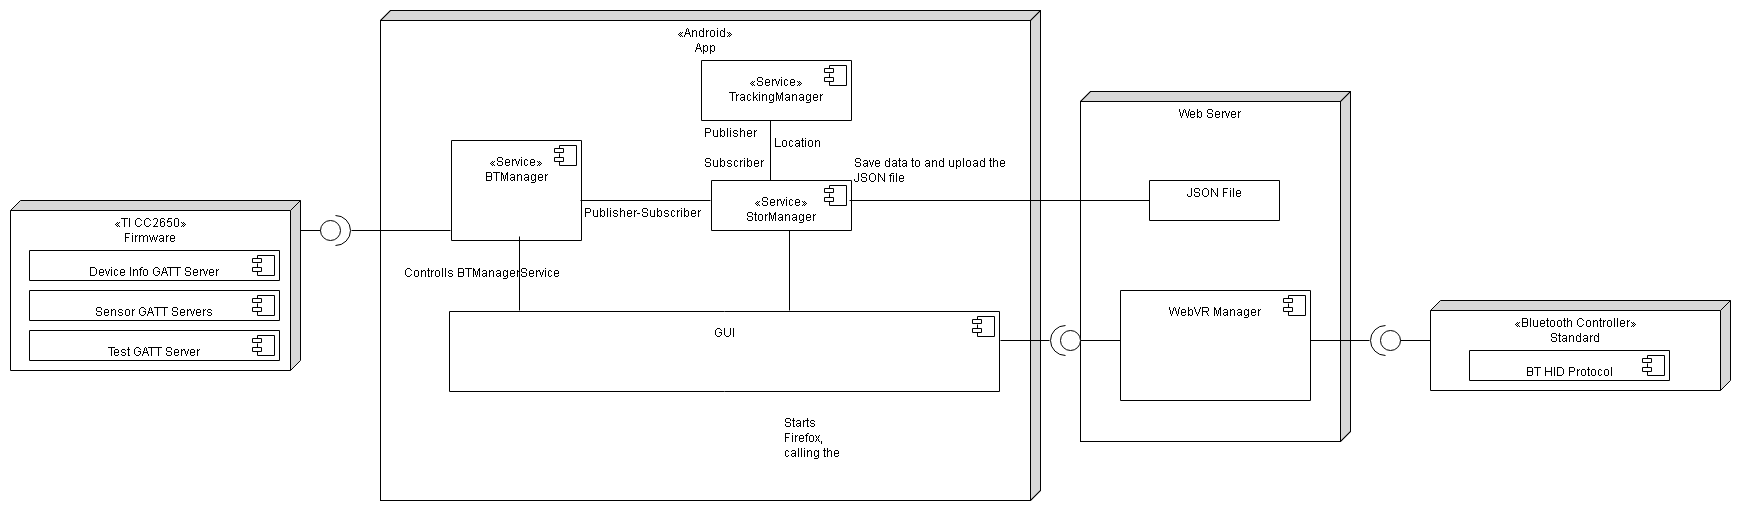
\includegraphics[width=1.4\textwidth]{pics/composite_app.png}


\subsection{Component Decomposition}

\subsubsection{Services}

\begin{itemize}
  \item \textbf{BluetoothLEService:} Uses the android.bluetooth and especially the android.bluetooth.le libraries to connect to a TI CC2650 MCU, fetch the sensor data from the MCU, to convert those values and broadcast them. \\

 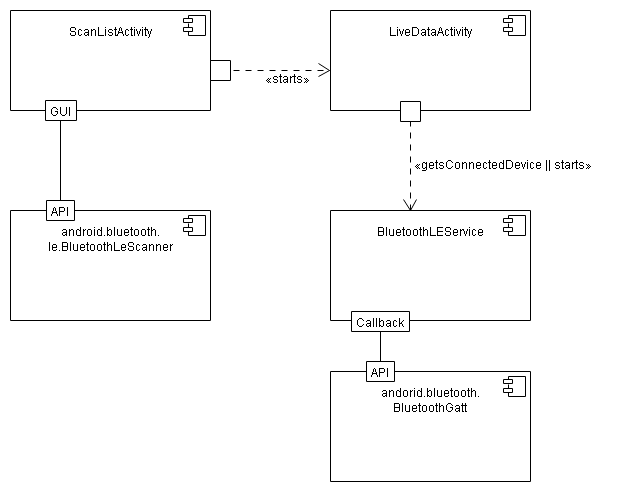
\includegraphics[width=0.8\textwidth]{pics/ble_man.png}

  \item \textbf{TrackingManager:} Handles the tracking of the (current) location where the data are recorded. The current position is determined by GPS and enhanced by the cellphone sensor and wifi data.

 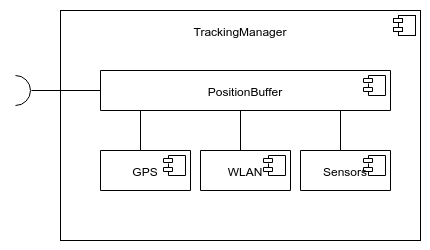
\includegraphics[width=0.8\textwidth]{pics/TrackingManager_Composition.png}

  \item \textbf{StorageManager:} Processes the data provided by the TrackingManager and the BluetoothManager. Uses a JSON file to store data.

 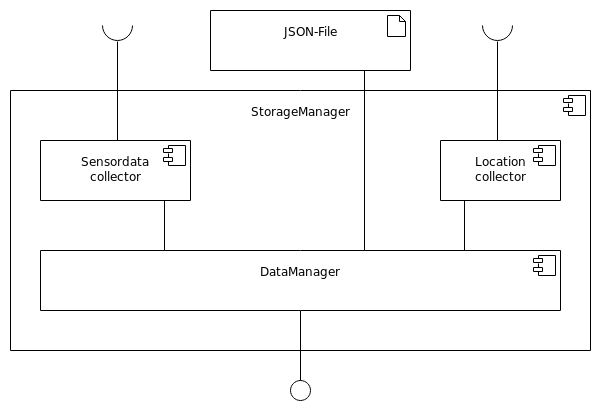
\includegraphics[width=0.8\textwidth]{pics/StorageMgr_Composition.png}

  \item \textbf{WebVRManager:} Handles the display of the virtual reality scene and the given data from the sensor.

 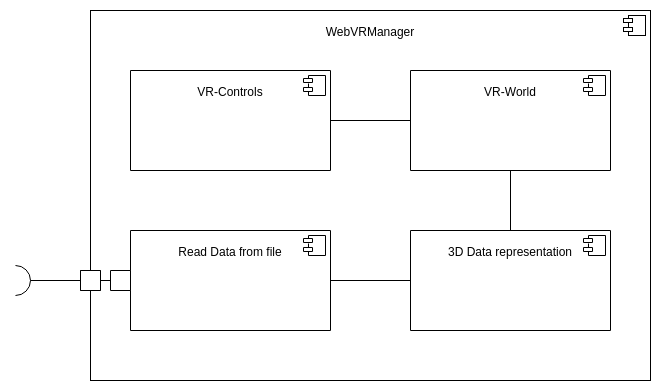
\includegraphics[width=0.8\textwidth]{pics/WebVRManager.png}

\end{itemize}

\subsubsection{GUI}

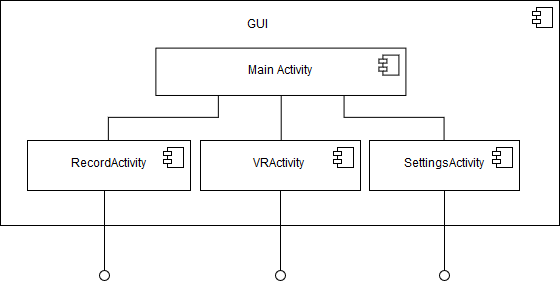
\includegraphics[width=0.8\textwidth]{pics/GUI-component.png}

\begin{itemize} % TODO
  \item \textbf{SplashActivity} Provides the main startup screen as the main entry point.
  \item \textbf{MainActivity} Provides the main startup screen as the main entry point.
  \item \textbf{RecordActivity} Provides an user interface to record new data.
  \item \textbf{SessionActivity} Provides an user interface to record new data.
  \item \textbf{LiveDataActivity} Shows the data that are received in real time using the android databinding api
  \item \textbf{SettingsActivity} Provides a user interface to configure the connectivity to the sensor device and the tracking options.
  \item \textbf{ScanListActivity} Used to start the scan and to let the user initiate the connection routine(s)
\end{itemize}

\subsubsection{Additional Classes}
\begin{itemize}
  \item \textbf{TIUUIDs} GATT TI CC2650 Service UUIDs
  \item \textbf{Sensor} Parser and helper functions for each sensor because the BLE protocol implemented in the TI CC2650 delivers raw sensor output
  \item \textbf{SensorDataListAdapter, LeDeviceAdapter, ScanListItem, DataListItem} Adapters, data- and view holders for the databinding api
\end{itemize}

\subsection{Hardware/ Software mapping}

The product consists of two parts which both run on the smart phone: \\
Firstly, the app will connect to the bluetooth sensor, gather the data and store them on a web server. \\
Secondly, the web application will also run on the smart phone and will be executed in a web browser which can be started by the user from within the app. The web application will show a previously built scene and display the gathered sensor's data in virtual reality.

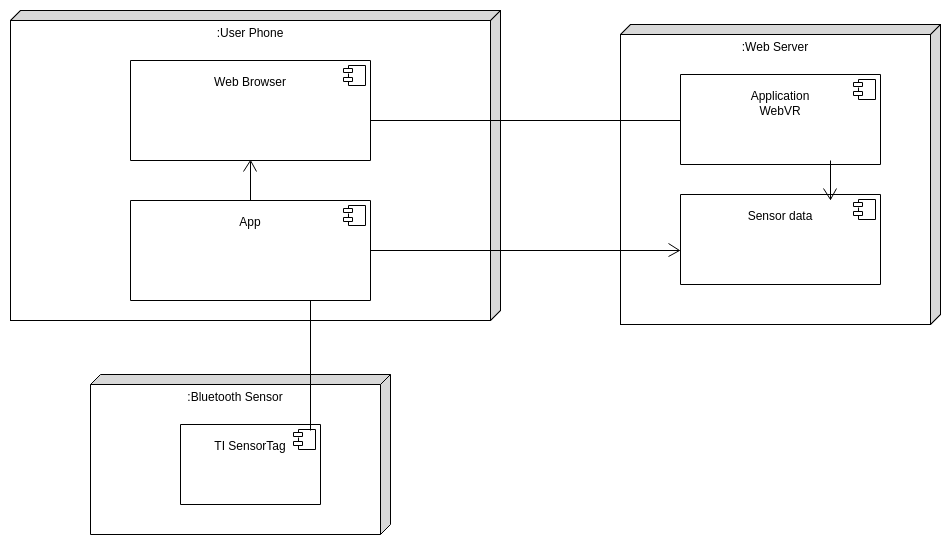
\includegraphics[width=0.8\textwidth]{diagramms/hsMapping.png}


\subsection{Global software control}
\subsubsection{Startup behavior}
\textbf{User:} The user can start the app by pressing the icon on his screen.
The app will show a startup screen and then transition after a short time into the main menu, from where the user can start the other functions of the app.

\subsubsection{Interfaces}
    The \textbf{BluetoothManager} provides a possibility to connect to a sensor and then record
    the data. It ensures that a connection is established and that the data are broadcasted via a local BroadcastManager. The first listing below contains the names of the intents and what extra data they contains. The second one lists the interfaces of the ServiceConnection, that's used to bind the service. \\
    \begin{lstlisting}

      public enum Sensor {

          /**
           * Constructor and main fields;
           * there is also a constant byte code "ENABLE_CODE" = 0000 0001
           * @param name the name of the according sensor
           * @param service The UUID of the GATT Service of the sensor
           * @param data The UUID of the Characteristic of the sensor data
           * @param config The UUID of the configuration characteristic
           */
         Sensor(String name, UUID service, UUID data, UUID config);

         /**
          * Used to convert the received binary values into human readable form
          *
          * @param the raw byte value of the received Bluetooth characteristic
          */
         public float convert(byte[] value) {
          requires value != null
            ensures correctly conversion from byte to value in human-readable format
         }

      }
    \end{lstlisting}
    \begin{lstlisting}
      /**
       * This abstract class is used to implement {@link BluetoothGatt} callbacks.
       */
      public class BluetoothLEService extends Service {

            /**
             * Methods overridden from the interface android.app.service
             */

             /**
               * Called by the system every time a client explicitly starts the service by calling
               * {@link android.content.Context#startService}, providing the arguments it supplied and a
               * unique integer token representing the start request.  Do not call this method directly.
               *
               * <p>For backwards compatibility, the default implementation calls
               * {@link #onStart} and returns either {@link #START_STICKY}
               * or {@link #START_STICKY_COMPATIBILITY}.
               *
               * <p>If you need your application to run on platform versions prior to API
               * level 5, you can use the following model to handle the older {@link #onStart}
               * callback in that case.  The <code>handleCommand</code> method is implemented by
               * you as appropriate:
               *
               * {@sample development/samples/ApiDemos/src/com/example/android/apis/app/ForegroundService.java
               *   start_compatibility}
               *
               * Note that the system calls this on your
               * service's main thread.  A service's main thread is the same
               * thread where UI operations take place for Activities running in the
               * same process.  You should always avoid stalling the main
               * thread's event loop.  When doing long-running operations,
               * network calls, or heavy disk I/O, you should kick off a new
               * thread, or use {@link android.os.AsyncTask}.</p>
               *
               * @param intent The Intent supplied to {@link android.content.Context#startService},
               * as given.  This may be null if the service is being restarted after
               * its process has gone away, and it had previously returned anything
               * except {@link #START_STICKY_COMPATIBILITY}.
               * @param flags Additional data about this start request.  Currently either
               * 0, {@link #START_FLAG_REDELIVERY}, or {@link #START_FLAG_RETRY}.
               * @param startId A unique integer representing this specific request to
               * start.  Use with {@link #stopSelfResult(int)}.
               *
               * @return The return value indicates what semantics the system should
               * use for the service's current started state.  It may be one of the
               * constants associated with the {@link #START_CONTINUATION_MASK} bits.
               *
               * @see #stopSelfResult(int)
               */
            public int onStartCommand(Intent, int, int);

            /**
             * Called by the system to notify a Service that it is no longer used and is being removed.  The
             * service should clean up any resources it holds (threads, registered
             * receivers, etc) at this point.  Upon return, there will be no more calls
             * in to this Service object and it is effectively dead.  Do not call this method directly.
             */
            public void onDestroy();

            /**
              * Return the communication channel to the service.  May return null if
              * clients can not bind to the service.  The returned
              * {@link android.os.IBinder} is usually for a complex interface
              * that has been described using
              * aidl.
              *
              * <p><em>Note that unlike other application components, calls on to the
              * IBinder interface returned here may not happen on the main thread
              * of the process</em>.  More information about the main thread can be found in
              * Processes and
              * Threads.</p>
              *
              * @param intent The Intent that was used to bind to this service,
              * as given to {@link android.content.Context#bindService
              * Context.bindService}.  Note that any extras that were included with
              * the Intent at that point will <em>not</em> be seen here.
              *
              * @return Return an IBinder through which clients can call on to the
              *         service.
              */
            public void onBind(Intent);

            /**
             * Called when all clients have disconnected from a particular interface
             * published by the service.  The default implementation does nothing and
             * returns false.
             *
             * @param intent The Intent that was used to bind to this service,
             * as given to {@link android.content.Context#bindService
             * Context.bindService}.  Note that any extras that were included with
             * the Intent at that point will <em>not</em> be seen here.
             *
             * @return Return true if you would like to have the service's
             * {@link #onRebind} method later called when new clients bind to it.
             */
            public boolean onUnbind(Intent);


            public class BluetoothGattCallback {

              /**
               * Callback indicating when GATT client has connected/disconnected to/from a remote
               * GATT server.
               */
              public void onConnectionStateChange(BluetoothGatt gatt, int status,
                                                  int newState) {
                ensures sending a broadcast containing the state information
              }

              /**
               * Callback invoked when the list of remote services, characteristics and descriptors
               * for the remote device have been updated, ie new services have been discovered.
               *
               * @param gatt GATT client invoked {@link BluetoothGatt#discoverServices}
               * @param status {@link BluetoothGatt#GATT_SUCCESS} if the remote device
               *               has been explored successfully.
               */
              public void onServicesDiscovered(BluetoothGatt gatt, int status) {
              }

              /**
               * Callback reporting the result of a characteristic read operation.
               *
               * @param gatt GATT client invoked {@link BluetoothGatt#readCharacteristic}
               * @param characteristic Characteristic that was read from the associated
               *                       remote device.
               * @param status {@link BluetoothGatt#GATT_SUCCESS} if the read operation
               *               was completed successfully.
               */
              public void onCharacteristicRead(BluetoothGatt gatt, BluetoothGattCharacteristic characteristic,
                                               int status) {
              }

              /**
               * Callback indicating the result of a characteristic write operation.
               *
               * <p>If this callback is invoked while a reliable write transaction is
               * in progress, the value of the characteristic represents the value
               * reported by the remote device. An application should compare this
               * value to the desired value to be written. If the values don't match,
               * the application must abort the reliable write transaction.
               *
               * @param gatt GATT client invoked {@link BluetoothGatt#writeCharacteristic}
               * @param characteristic Characteristic that was written to the associated
               *                       remote device.
               * @param status The result of the write operation
               *               {@link BluetoothGatt#GATT_SUCCESS} if the operation succeeds.
               */
              public void onCharacteristicWrite(BluetoothGatt gatt,
                                                BluetoothGattCharacteristic characteristic, int status) {
              }

              /**
               * Callback triggered as a result of a remote characteristic notification.
               *
               * @param gatt GATT client the characteristic is associated with
               * @param characteristic Characteristic that has been updated as a result
               *                       of a remote notification event.
               */
              public void onCharacteristicChanged(BluetoothGatt gatt,
                                                  BluetoothGattCharacteristic characteristic) {
              }


              /**
               * Callback indicating the result of a descriptor write operation.
               *
               * @param gatt GATT client invoked {@link BluetoothGatt#writeDescriptor}
               * @param descriptor Descriptor that was writte to the associated
               *                   remote device.
               * @param status The result of the write operation
               *               {@link BluetoothGatt#GATT_SUCCESS} if the operation succeeds.
               */
              public void onDescriptorWrite(BluetoothGatt gatt, BluetoothGattDescriptor descriptor,
                                            int status) {
              }

              /**
               * Callback reporting the RSSI for a remote device connection.
               *
               * This callback is triggered in response to the
               * readRemoteRssi function.
               *
               * @param gatt GATT client invoked {@link BluetoothGatt#readRemoteRssi}
               * @param rssi The RSSI value for the remote device
               * @param status {@link BluetoothGatt#GATT_SUCCESS} if the RSSI was read successfully
               */
              public void onReadRemoteRssi(BluetoothGatt gatt, int rssi, int status) {
              }

              /**
               * Broadcasts the converted Bluetooth characteristic that was read from the sensor.
               *
               * @param characteristic Characteristic that has been received from a sensor.
               */
              private void broadcastCharacteristic(BluetoothGattCharacteristic characteristic) {
              }
            }

            /**
             * connects through the gatt callback to a  TI CC2650 MCU using its MAC-address
             *
             * @param the MAC address of a TI CC2650 MCU
             */
            public boolean connect(String address) {
              requires address != null
                ensures established connection to the device
            }

            public void disconnect() {
              ensures disconnection from a connected TI CC2650 MCU
            }

            /**
             * Basic sensor control: turn power and notifications on and off.
             *
             * @param s            Sensor enum: IR_TEMPERATURE || BAROMETER || LUXMETER || HUMIDITY
             * @param power        true = on, false=off
             * @param notification true = enabled, false=off
             */
            private void controlSensor(Sensor s, boolean power, boolean notification) {
             }

            /**
             * Wrapper for a blocking write: Either execute if the Queue is empty and no write is currently
             * going on or enqueue the write task.
             *
             * @param o Either a BluetoothGATTCharacteristic (e.g. the config characteristic to turn the
             *          sensor on and off) or a BluetoothGattDescriptor (e.g. the Client Characteristic
             *          Config descriptor, to en-/disable the notifications).
             */
            private synchronized void write(Object o) {
            }

            /**
             * Blocking write; Sets isWriting to true (onWriteCharacteristic/Descriptor settings it to false when
             * finished)
             *
             * @param o Either a BluetoothGATTCharacteristic (e.g. the config characteristic to turn the
             *          sensor on and off) or a BluetoothGattDescriptor (e.g. the Client Characteristic
             *          Config descriptor, to en-/disable the notifications).
             */
            private synchronized void doWrite(Object o) {
            }

            /**
             * Function that is called if a write finishes or has illegal arguments
             */
            private synchronized void nextWrite() {
            }

      }
    \end{lstlisting}
    \begin{lstlisting}
      public class ScanListActivity extends AppCompatActivity {

          /**
           * Methods overridden from the interface import android.support.v7.app.AppCompatActivity;
           */

          /**
            * Called when the activity is starting.  This is where most initialization
            * should go: calling {@link #setContentView(int)} to inflate the
            * activity's UI, using {@link #findViewById} to programmatically interact
            * with widgets in the UI, calling
            * {@link #managedQuery(android.net.Uri , String[], String, String[], String)} to retrieve
            * cursors for data being displayed, etc.
            *
            * <p>You can call {@link #finish} from within this function, in
            * which case onDestroy() will be immediately called without any of the rest
            * of the activity lifecycle ({@link #onStart}, {@link #onResume},
            * {@link #onPause}, etc) executing.
            *
            * <p><em>Derived classes must call through to the super class's
            * implementation of this method.  If they do not, an exception will be
            * thrown.</em></p>
            *
            * @param savedInstanceState If the activity is being re-initialized after
            *     previously being shut down then this Bundle contains the data it most
            *     recently supplied in {@link #onSaveInstanceState}.  <b><i>Note: Otherwise it is null.</i></b>
            *
            */
          protected void onCreate(Bundle savedInstanceState) {
          }

          /**
           * Dispatch onResume() to fragments.  Note that for better inter-operation
           * with older versions of the platform, at the point of this call the
           * fragments attached to the activity are <em>not</em> resumed.  This means
           * that in some cases the previous state may still be saved, not allowing
           * fragment transactions that modify the state.  To correctly interact
           * with fragments in their proper state, you should instead override
           * {@link #onResumeFragments()}.
           */
          protected void onResume() {
          }

          /**
            * Called as part of the activity lifecycle when an activity is going into
            * the background, but has not (yet) been killed.  The counterpart to
            * {@link #onResume}.
            *
            * <p>When activity B is launched in front of activity A, this callback will
            * be invoked on A.  B will not be created until A's {@link #onPause} returns,
            * so be sure to not do anything lengthy here.
            *
            * <p>This callback is mostly used for saving any persistent state the
            * activity is editing, to present a "edit in place" model to the user and
            * making sure nothing is lost if there are not enough resources to start
            * the new activity without first killing this one.  This is also a good
            * place to do things like stop animations and other things that consume a
            * noticeable amount of CPU in order to make the switch to the next activity
            * as fast as possible, or to close resources that are exclusive access
            * such as the camera.
            *
            * <p>In situations where the system needs more memory it may kill paused
            * processes to reclaim resources.  Because of this, you should be sure
            * that all of your state is saved by the time you return from
            * this function.  In general {@link #onSaveInstanceState} is used to save
            * per-instance state in the activity and this method is used to store
            * global persistent data (in content providers, files, etc.)
            *
            * <p>After receiving this call you will usually receive a following call
            * to {@link #onStop} (after the next activity has been resumed and
            * displayed), however in some cases there will be a direct call back to
            * {@link #onResume} without going through the stopped state.
            *
            * <p><em>Derived classes must call through to the super class's
            * implementation of this method.  If they do not, an exception will be
            * thrown.</em></p>
            */
         protected void onPause() {
           }

          /**
           * Bluetooth LE scan callbacks. Scan results are reported using these callbacks.
           *
           * @see BluetoothLeScanner#startScan
           */
          public abstract class ScanCallback {
              /**
               * Callback when a BLE advertisement has been found.
               *
               * @param callbackType Determines how this callback was triggered. Could be one of
               *            {@link ScanSettings#CALLBACK_TYPE_ALL_MATCHES},
               *            {@link ScanSettings#CALLBACK_TYPE_FIRST_MATCH} or
               *            {@link ScanSettings#CALLBACK_TYPE_MATCH_LOST}
               * @param result A Bluetooth LE scan result.
               */
              public void onScanResult(int callbackType, ScanResult result) {
              }

              /**
               * Callback when batch results are delivered.
               *
               * @param results List of scan results that are previously scanned.
               */
              public void onBatchScanResults(List<ScanResult> results) {
              }

              /**
               * Callback when scan could not be started.
               *
               * @param errorCode Error code (one of SCAN_FAILED_*) for scan failure.
               */
              public void onScanFailed(int errorCode) {
              }
          }

          /**
           * @param enable if true the scan will start and stop after 5 seconds
           *               if false the scan will stop immediately
           */
          private void scanLeDevice(final boolean enable) {
          }

      }
    \end{lstlisting}

    \noindent The \textbf{StorageManager} provides a possibility to store the data from the sensor together with the current position.
    It also can store the data in a .json file and upload them to a webserver.

    \begin{lstlisting}
    InterfaceStorageManager {
      public void setSensor(integer internalSensorID){
        activeSensor = internalSensorID;
      }
      //tells the storage manager to get data from the active sensor and
      //the tracing manager, mark them with a timestamp and store the data
      //in a DataSet.
      public void measureNow(){
      }
      //get the latest measured DataSet of the active sensor
      public DataSet getLiveData() {
        return DataSet;
      }
      //get a DataSet which contains data of the activeSensor and position
      //at the specified time. If no data was stored at that time, an empty
      //DataSet will be returned.
      public DataSet getDataFrom(int time) {
        return DataSet;
      }
      //get multiple DataSets which contain all measured Data from the
      //active Sensor between 'time' and now.
      public DataSet[] getDataSince(int time) {
        return DataSet[];
      }
      // Upload the data set to a webserver
      // a .json file from time till now.
      public void uploadData(int time) {
        //upload the data to a server so webvr can later use it.
      }
    }
    \end{lstlisting}


    The \textbf{TrackingManager} gets the current location of the smartphone and provides it to the rest of
    the App.

    \begin{lstlisting}
    Interface TrackingManager {
      //get the current location of the device
      public Location p getCurrentPosition() {
        ensures iff lockCustomPos
          p == customPos;
          else
            p == currentPosition;
      }
    }
    \end{lstlisting}


    The \textbf{VRBox} gets the data from a webserver and loads it into the VR-World.

    \begin{lstlisting}
    Interface WebVR {
      //Load the data from the webserver to display in VR.
      //The data will be a .json file which will be parsed
      // by in javascript by the web page.
      function loadData(file){
      }
    }
    \end{lstlisting}

\subsubsection{Sequences}

\begin{description}
	\item[1) Start VR view:] When the user clicks a button to start the VR view, a web browser is opened via an intent.  \\
	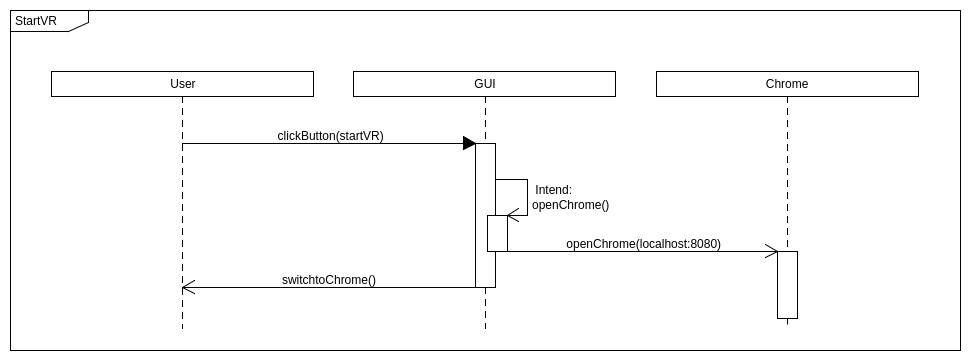
\includegraphics[width=0.8\textwidth]{diagramms/startVR.png}

	\item[2) Switch to stereoscopic 3D: ] When the user enters the VR view, he can choose to switch the view and thereby switch to a stereoscopic view or switch back to non-stereoscopic view, respectively. \\
	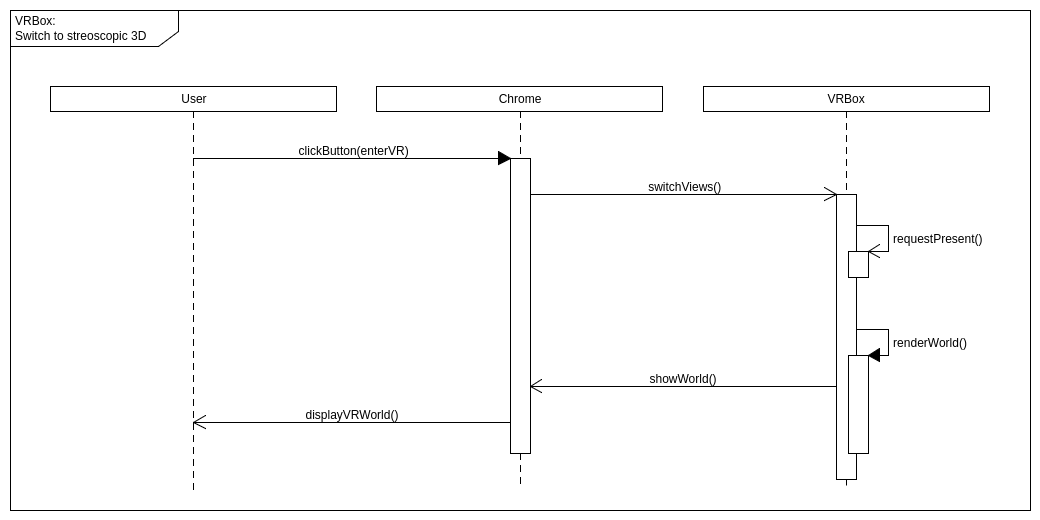
\includegraphics[width=0.8\textwidth]{diagramms/stereo.png}

	\item[3) Switch data visualization: ] When the user opens the web site with the VR view, he  can switch the visualization. The first view is a plane composed from
  the location tracking together with the data from the sensor, the second visualization is a representation of the locations as dots
  and the data as numbers hovering over these dots.  \\
	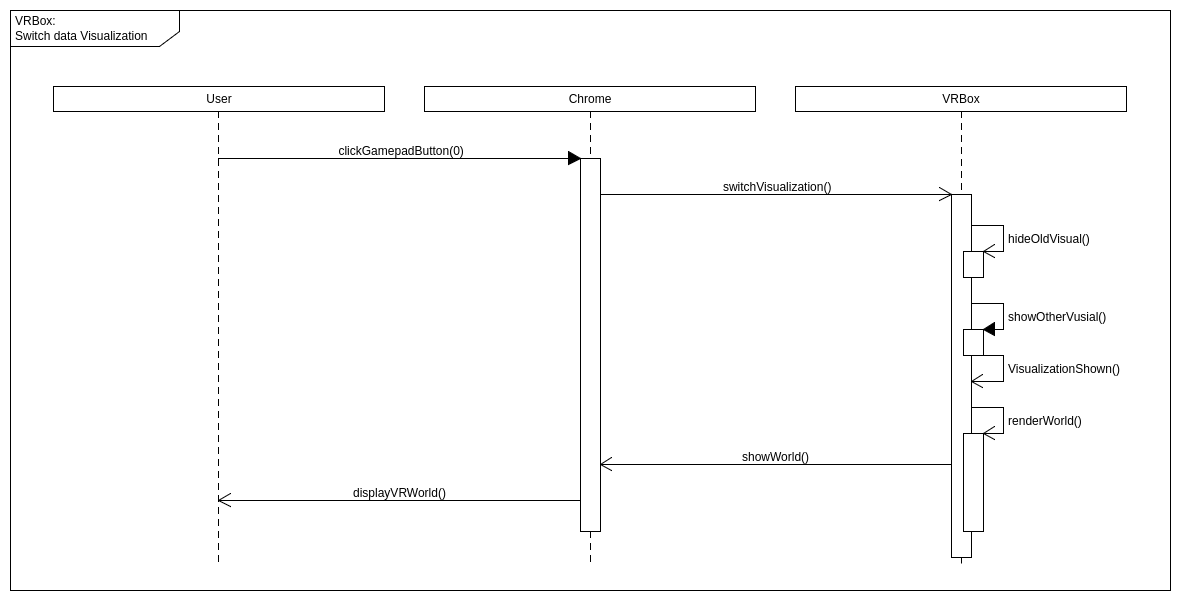
\includegraphics[width=0.8\textwidth]{diagramms/switchVisual.png}

	\item[4) Scan and Connect:] Scan for Bluetooth low energy devices and connect to one of them by clicking on the correct result ("TI CC2650").
	After beeing connected one can edit the configuration of the sensors on the CC2650: \\dis-/enable a sensor, (de-)activate the notifications for a measurement characteristic, read values, disconnect from the device. After that the user may start a new data scan record or start the VR View.\\
	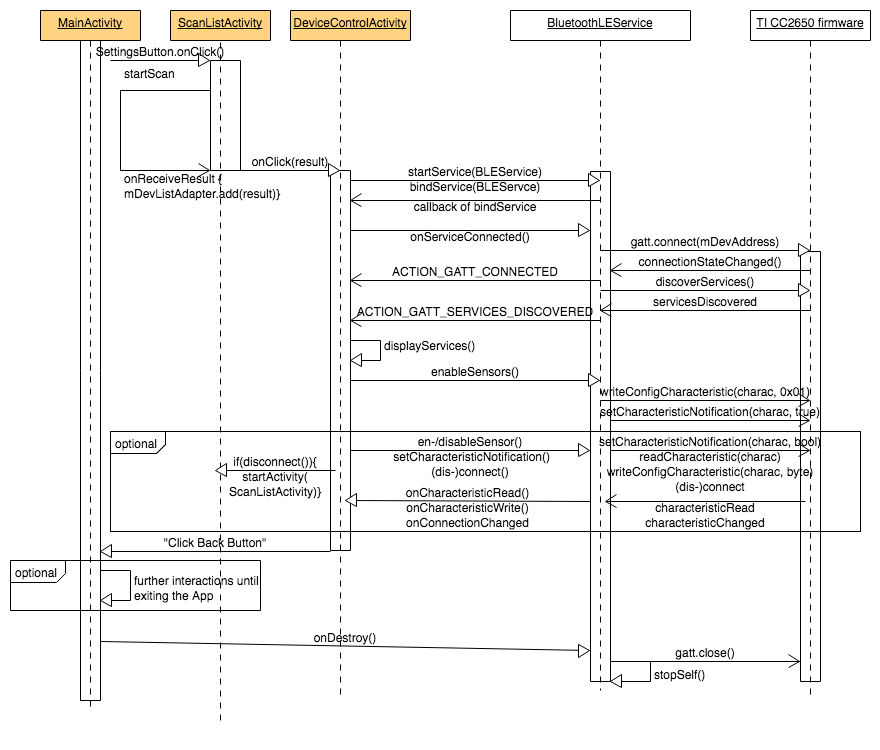
\includegraphics[width=0.8\textwidth]{diagramms/bleseq.png}

	\item[6) Record new data set: ] When the user clicks the button to record a new data set, the StorageManager will provide the data and get the repective location from the TrackingManager to calibrate the initial location for the recording session. \\
	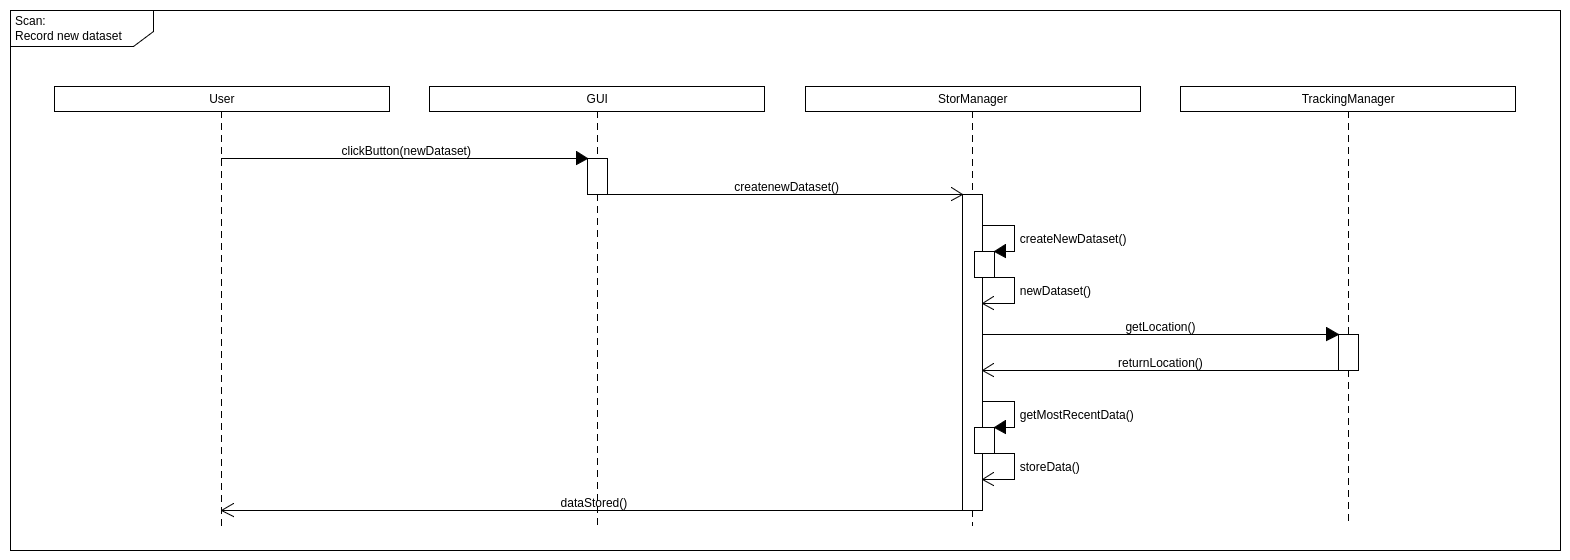
\includegraphics[width=0.8\textwidth]{diagramms/newDataset.png}

%	\item[7) Record data point: ] When the user clicks the button to record new data, the StorageManager will provide the data and get the repective location from the TrackingManager.\\
%	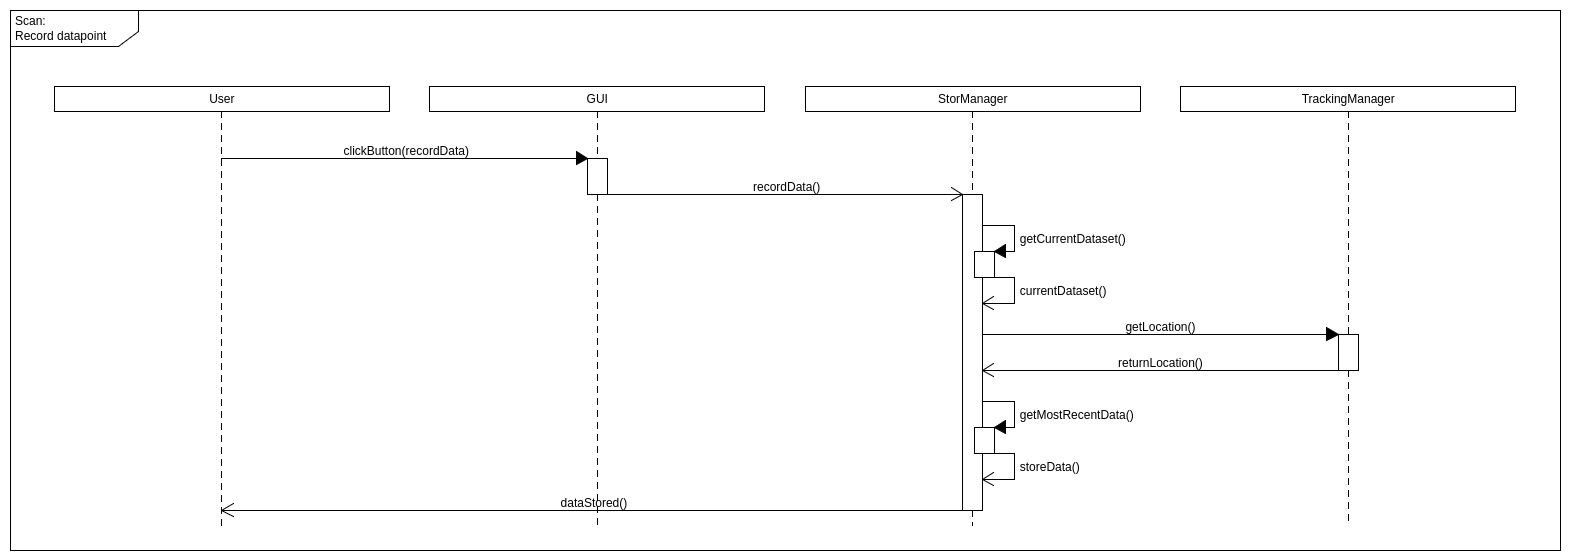
\includegraphics[width=0.8\textwidth]{diagramms/recordDatapoint.png}



\end{description}
